\section{Détails du sujet de stage}
\subsection{Présentation d'IDL}

\textbf{IDL} - Interactive Data Language est un langage interprété sous licence propriétaire. Créé en 1977 il a attiré l'attention des astronomes, médecins et d'autres scientifiques qui ont eu besoin d'un langage assez simple à apprendre et assez puissant pour traiter les données massives avec des fonctionnalités graphiques. La popularité d'\textbf{IDL} augmentait très vite à cause de ses fonctionnalités très pratiques pour les chercheurs, qui n'ont pas été programmeurs, mais qui ont besoin d'un outil pour faire des calculs scientifique. Entre ces fonctionnalités on trouve:

\begin{itemize}
	\item[$\bullet$] typage dynamique, le type est attribué automatiquement pendant la définition  de sa valeur (il y a une quinzaine de types);
	\item[$\bullet$] capacités d'un langage de programmation orientée objet;
	\item[$\bullet$] interprétation par machine virtuelle;
	\item[$\bullet$] affichage de tracés (1D, 2D, 3D) sans utilisation des bibliothèques graphiques externes;
	\item[$\bullet$] \textbf{IDL} est un langage vectorisé, les opérations sur scalaires sont généralisées pour pouvoir les utiliser sur les vecteurs, matrices et les tableaux à une dimension supérieure;
	\item[$\bullet$] multitâche, certaines fonctions et procédures sont parallélisés.
\end{itemize}

Grâce à ces avantages et une disponibilité sur les systèmes d'exploitations les plus utilisés y compris Windows, Mac OS X, Linux et Solaris, aujourd'hui il existe de nombreuses bibliothèques écrites complètement en syntaxe \textbf{IDL}. Ce sont les modules spécifiques à un domaine, qui ont été crées par les scientifiques pour simplifier l'utilisation de langage \textbf{IDL} dans ses domaines. Par exemple:  \textit{IDL Astronomy User's Library} ou plus court \textit{AstroLib} crée par Wayne Landsman. Cette bibliothèque contient des procédures fréquemment utilisées par les astronomes, notamment pour relire certaines formats de données (FITS).

\textbf{IDL} est un langage de programmation dont l’interpréteur du langage (ou compilateur) est propriétaire, ce qui signifie qu’il n’est pas libre. Cela signifie aussi que les scientifiques n’ont pas accès au code source et qu’il ne peuvent ouvrir qu’une quantité limitée de sessions au travers d’un système de jetons.

Le système de jetons dans \textbf{IDL} est contraignant. Déjà, l'abonnement pour un jeton par an coûte plus de 1000 \euro. En plus, il y a un nombre limité d’ouverture d’\textbf{IDL}, car à chaque démarrage du logiciel, ce dernier va réserver des jetons disponibles sur un serveur. Cela implique aussi que l’utilisateur doit rester connecté au serveur détenteur de jetons, ce qui peut très vite s’avérer compliqué en déplacement professionnel, durant des présentations ou lors de démonstration pendant des conférences.

Mais ce qui pose encore plus de problèmes aux scientifiques, c’est la pérennité du logiciel. En effet, ne pas avoir les codes source à disposition implique le fait que si la société en charge de garder le logiciel à jour décide de cesser ses activités, personne ne pourra continuer le développement. Dans le passé, la NASA et l'ESA ont contraint l’éditeur, qui voulait ne garder que Windows, à poursuivre le developpement sous Mac OS X et Linux. Or, la technique évolue tous les jours, et les logiciels tels qu'est \textbf{IDL} se doivent de la suivre. De plus, s’il n’est plus possible d’utiliser \textbf{IDL} dans le futur, les nombreuses bibliothèques écrites en syntaxe \textbf{IDL} deviendront inutiles et il faudra recoder tous les algorithmes dans un autre langage de programmation, ce qui serait très long et extrêmement cher. %\\

\subsection{Présentation de GDL}

\textbf{GDL} - GNU Data Language est un compilateur libre compatible avec la syntaxe \textbf{IDL}. Il a été créé par Marc Schellens en 2004 et il est développé par une communauté internationale de volontaires. \textbf{GDL} a été créé pour bénéficier des avantages d'\textbf{IDL} en ajoutant la liberté de compilateur pour assurer la pérennité de logiciel lui même et les bibliothèques tierces écrites en syntaxe \textbf{IDL}. L’interprétation de syntaxe est basé sur ANTLR.

\textbf{GDL} est déjà une alternative viable couvrant la plupart des fonctionnalités d'\textbf{IDL} et peut être utilisé pour compiler de larges "pipelines" de codes et bibliothèques en syntaxe \textbf{IDL}, lire les donnée de divers formats utilisées par les scientifiques (comme FITS, HDF, NetCDF, XDR), faire des calculs complexes et retourner un résultat exact. Grâce aux packagers les versions pré-compilées et pré-configurées sont mise à disposition pour les distribution de Linux les plus populaires (Debian, Ubuntu, Fedora, Gentoo, ArchLinux\ldots), FreeBSD et Mac OS X. Pour les utilisateurs plus expérimentés la version la plus récente du code est disponible sue un CVS (accès an lecture seul à tous), qui peut être compilée sur presque tous les systèmes basés sur Unix.

La compatibilité avec Windows n'est pas assurée, mais toutes les nouveau fonctionnalités prennent en compte la compatibilité avec ce système et les fonctionnalités déjà présent dans \textbf{GDL} continuent d'évoluer pour être compatibles avec tous les systèmes possibles.

\begin{figure}[!ht]
    \centerline{
    	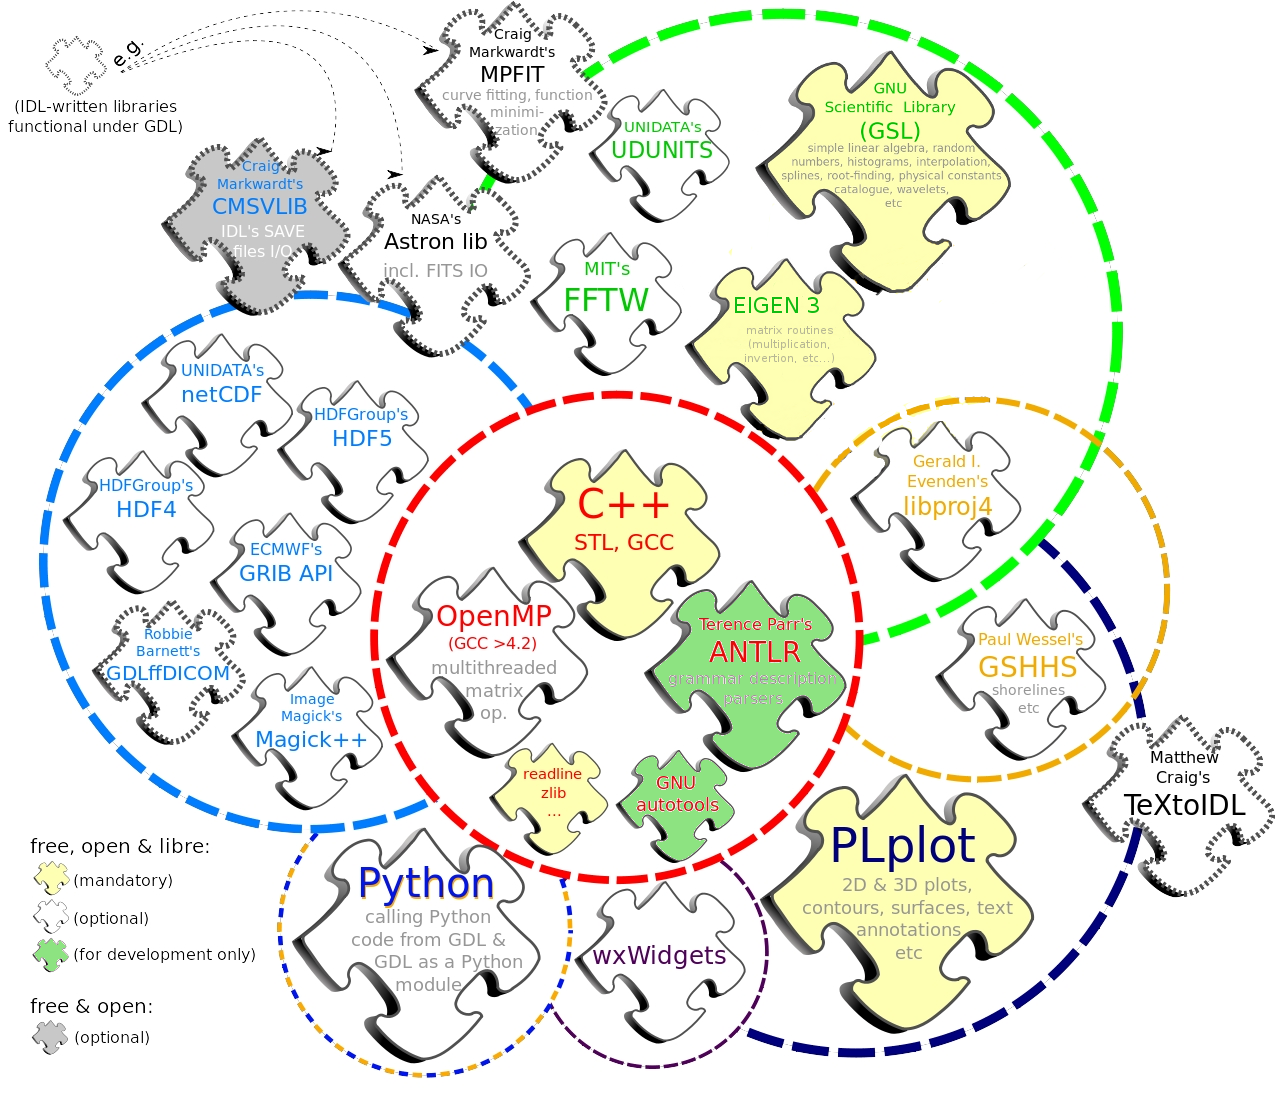
\includegraphics[width=1.3\textwidth]{./images/gdl-mod.png}
    	}
    \caption{Dépendances de GDL}
    \label{gdl-dep}
\end{figure}
%\newpage
Le choix de bonnes librairies externes et de bons algorithmes internes, l'usage de OpenMP, donnent une bonne performance globale à GDL. Sur les multi-cœurs, les gaines attendus sont généralement constatés. Les tests de performances actuels montrent que les calculs avec \textbf{GDL} sont aussi rapides (parfois plus vite), que les calculs avec son  adversaire propriétaire et ce, en respectant le gain par nombre de cœurs. L'ultime déficience connue dans le benchmarck de référence (IDL TIME\_TEST\_4) est SMOOTH, sujet du second stagiaire.
%\newpage
Le plus grand inconvénient de \textbf{GDL} est l'absence de plusieurs fonctions et procédures présentes dans \textbf{IDL}, alors ma mission a été de diminuer le nombre de ces fonctions/procédures manquantes et de tester ces nouvelles fonctionnalités en comparant les performances de \textbf{GDL} et d'\textbf{IDL}.

Le projet \textbf{GDL} utilise la licence GNU GPL v2/v3. Les bibliothèques tierces utilisée dans ce projet sont uniquement des bibliothèques libres (la notion d'un logiciel libre/licence libre est définie dans la section \ref{log_lib}, page \pageref{log_lib}) avec la licence GPL ou un autre, compatible avec GPL. Une exception unique concerne une fonctionnalité importante d'un format propriétaire de fichier interne à \textbf{IDL}. Il se trouve qu'une librairie externe open source à la licence incompatible avec la GNU GPL permet de gérer ce format. Il revient à l'utilisateur d'ajouter lui même ce code.



\subsection{Logiciel libre}
\label{log_lib}


La notion de Logiciel Libre (Free Software) est inventée par Richard Stallman dans le début des années 1980. Une première définition est publiée en 1986 par FSF (Free Software Foundation), une organisation américaine à but non lucratif, dont la mission mondiale est la promotion du logiciel libre et la défense des utilisateurs. Cette définition se traduit par une tente d'une licence définissant les droits et les devoirs des utilisateurs en s'appuyant sur le droit d'auteur (Copyright). Rarement, la FSF modifie la notion de Logiciel libre afin de la clarifier ou pour résoudre des questions portant sur des points difficiles. Les deux principales licences GNU GPL sont les versions 2 et 3.

Selon la dernière définition, un programme est un logiciel libre si, en tant qu'utilisateur de ce programme, vous avez les quatre libertés essentielles:

\begin{description}
	\item[liberté 0]  \hfill \\ %[$\bullet$] \textbf{liberté 0:} 
la liberté d'exécuter le programme, pour tous les usages;
	\item[liberté 1]  \hfill \\  %[$\bullet$] \textbf{liberté 1:} 
la liberté d'étudier le fonctionnement du programme, et de le modifier pour qu'il effectue vos tâches informatiques comme vous le souhaitez; l'accès au code source est une condition nécessaire ;
	\item[liberté 2]  \hfill \\ %[$\bullet$] \textbf{liberté 2:} 
la liberté de redistribuer des copies, donc d'aider votre voisin;
	\item[liberté 3]   \hfill \\ %[$\bullet$] \textbf{liberté 3:} 
la liberté de distribuer aux autres des copies de vos versions modifiées; en faisant cela, vous donnez à toute la communauté une possibilité de profiter de vos changements ; l'accès au code source est une condition nécessaire.
\end{description}



Pour protéger la [non]liberté d'un logiciel et les droit d'utilisateur il existe plusieurs type de licences. La FSF classe les licences en trois catégories :

\begin{itemize}
	\item[$\bullet$] les licences libres compatibles avec GPL;
	\item[$\bullet$] les licences libres non compatibles avec GPL;
	\item[$\bullet$] les licences non libres/propriétaires.
\end{itemize}

\begin{figure}[!ht]
    \centerline{
    	
\includegraphics[width=0.4\textwidth]{./images/GPLv3_Logo.png}
    	}
    \caption{Logo de GPL version 3}
    \label{logo-gpl}
\end{figure}
\begin{description}

\item[GNU General Public License]\hfill \\
La Licence Publique Générale GNU (GNU GPL ou GPL) est une licence des logiciels libres. Elle a été créé par Richard Stallman en 1989 pour permettre au grand nombre de projets de partager leur code source. C'est la licence le plus utilisée dans le monde de logiciels libres. La dernière version est "GNU GPL version 3" publiée en 2007. Ses termes autorisent l'utilisateur de logiciel sous licence GPL à: distribuer ce logiciel, le modifier, distribuer la version modifié. L'utilisateur n'est pas autorisé à: changer la licence, distribuer ce logiciel sans code source, commercialiser ce logiciel.

Ce ne signifie pas qu'on peut pas faire de l'argent avec les logiciels libres. L’entreprise multi-nationale Red Hat avec un chiffre d’affaire d'un milliard de dollars est dédiée aux logiciels libre et Open Source, qui a basé son modèle d'affaires sur la vente des services et supporte pour les logiciels libres, notamment le noyau Linux et le système d'exploitation RHEL (Red Hat Enterprise Linux).

\item[Berkeley software distribution license]\hfill \\
La licence BSD est une licence libre compatible avec la GPL. Ses termes sont moins restrictives que celles de GPL. Un logiciel sous licence BSD en différence de GPL peut être utilisé dans un autre projet commercial et l’accès au code source modifié n'est pas garanti.

\item[End User License Agreement]\hfill \\
Contrat de Licence Utilisateur Final est un licence non libre/propriétaire, ses termes sont définis par l’entreprise publiant le logiciel. Il est utilisé pour mettre les différent restrictions (restriction de distribution; restriction sur le nombre d'utilisateurs, qui peuvent utiliser ce logiciel).
\end{description}
